\testCom
{%Номер задачи
	3.173
}
{%Условие
	условие\\
}
{%Дано
	дано\\
}
{%Найти
	найти\\
}
{%Решение
	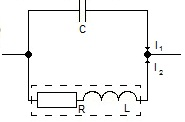
\includegraphics[height=30mm]{3_173.jpg}\\
	Правило Киргофа:\\
	$I_1 X_c = I_2 (R + X_L) = U$\\
	$I = I_1 + I_2, I Z = U$\\
	$Z= \frac{U}{I_1 + I_2}, \frac{1}{Z} = \frac{I_1}{U} \frac{X_1}{X_c} + \frac{I_2 (R + X_L)}{(R + X_L) U} =$\\
	$= \frac{1}{X_c} + \frac{1}{X_L + R}$\\
	$\frac{1}{X_c} + \frac{1}{R + X_L} = \frac{X_c + R + X_L}{X_c (R + X_L)}$\\
	$\abs{Z} = \frac{\abs{X_c} \cdot \abs{R + X_L}}{\abs{X_C + R + X_L}} = \frac{\sqrt{R^2 + \omega^2 L^2}}{\sqrt{(\omega R C)^2 + (1 - \omega^2 C L)^2}}$\\
	
}

